\documentclass[tikz]{standalone}
\usepackage{amsmath}
\usetikzlibrary{arrows,calc}
\begin{document}
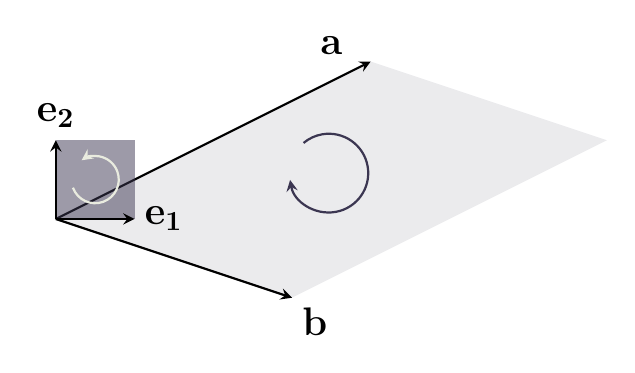
\begin{tikzpicture}[scale=1.0]
% ------------------------------------------------ lin_alg theme colors
\definecolor{la_white}{RGB}{233,235,223} %#E9EBDF
\definecolor{la_dark}{RGB}{59,54,81}     %#3B3651
\definecolor{la_gray}{RGB}{96,112,139}   %#60708B
\definecolor{la_tan}{RGB}{152,159,122}   %#989F7A

\def\centerarc[#1](#2)(#3:#4:#5)% Syntax: [draw options] (center) (initial angle:final angle:radius)
    { \draw[#1] ($(#2)+({#5*cos(#3)},{#5*sin(#3)})$) arc (#3:#4:#5); }

%\coordinate (c1) at (0,0);
\newcommand{\cercle}[5]{
\node[circle,inner sep=0,minimum size={2*#3}](a) at (#2) {};
\draw[#1] (a.#4) arc (#4:{#4+#5}:#3) ;
}
\cercle{thick,la_dark,>=stealth,<-}{3,0.5}{0.5}{190}{300};

\fill[color=la_dark,fill=la_dark,fill opacity=0.1] (0,0) -- (4,2) -- (7,1) -- (3,-1) -- cycle ;
\draw [thick,>=stealth,->] (0,0) -- (4,2)  node[yshift=2mm, xshift=-5mm] {\Large $\mathbf{a}$} ;
\draw [thick,>=stealth,->] (0,0) -- (3,-1) node[anchor=north west] {\Large $\mathbf{b}$} ;

\fill[color=la_gray,fill=la_dark,fill opacity=0.5] (0,0) rectangle (1,1) ;
\draw [thick,>=stealth,->] (0,0) -- (1,0)  node[anchor=west] {\Large $\mathbf{e_1}$} ;
\draw [thick,>=stealth,->] (0,0) -- (0,1)  node[anchor=north,yshift=6mm] {\Large $\mathbf{e_2}$} ;

%\centerarc[thick,color=black,>=stealth,->] (0.5,0.5) (-160:125:0.3) ;
\draw[thick,la_white,>=stealth,->] ([shift=(-160:0.3)]0.5,0.5) arc (-160:125:0.3);

\end{tikzpicture}
\end{document}